%% ============================================================
%% 分片 26：原文第 10 节「The Bogomolny Equations And The Space Of Hecke Modifications」（原文 glshort.tex 起于第 8120 行）
%% 由 tools/harvmac2tex.py 从 arXiv 源码（hep-th/0604151v3）自动生成。
%% 只译英文散文；公式、编号、\label、\cite 一律不改。
%% ============================================================

\section{Bogomolny 方程与 Hecke 修正的空间}

\label{sec:bogeqheck}

\begin{keytakeaways}
  \begin{itemize}[leftmargin=1.4em,itemsep=2pt,topsep=2pt]
    \item \textbf{物理图像}：给定型 $^L\negthinspace w$ 的 Hecke 修正空间，可以呈现为三维流形 $W=I\times C$ 上带 't Hooft 算子奇点、并带适当椭圆边界条件的 Bogomolny 方程解模空间。$E_-$ 端固定联络 $A_-$（Dirichlet）而让 $\phi_0$ 自由，$E_+$ 端令 $\phi_0=0$（协变 Neumann）而让 $A$ 自由；交换两端的保向自同构 ${\cal PT}$ 同时反转时间坐标。
    \item \textbf{数学工具}：指标理论。Bogomolny 方程线性化给出椭圆复形 $0\to\Omega^0({\rm ad}(E))\to\Omega^1({\rm ad}(E))\oplus\Omega^0({\rm ad}(E))\to\Omega^2({\rm ad}(E))\to 0$，其指标即模空间的虚拟维数；Pauly 借助 Kronheimer 的 $U(1)$-不变瞬子与等变指标定理，把奇点的贡献化为不动点的贡献。
    \item \textbf{关键结论}：Hecke 修正空间的复维数 $\Delta$ 等于各 't Hooft 算子贡献之和 $\Delta=\sum_i\Delta_{\rho_i}$；无算子时维数为零，单个 $T(\rho)$ 时 $\Delta_\rho=\sum_k c_k$。对 $G=PSU(2)$、最高权 $(a/2,-a/2)$ 贡献为 $a$，与第~\ref{sec:spaceheck}~节的维数公式一致，并推广到任意紧 Lie 群 $G$。
    \item \textbf{边界与展望}：指标理论只给出（虚拟）维数，不直接构造模空间；要定义任意 $A$-膜的 Hecke 变换并用于几何 Langlands 对偶，还需放弃时间反演不变性、改用复化（扩展）的 Bogomolny 方程。
  \end{itemize}
\end{keytakeaways}

本节中，我们回到带奇点的 Bogomolny 方程，更仔细地研究它们。第一个目标是把给定型的 Hecke 修正空间呈现为带适当边界条件的 Bogomolny 方程解的模空间。这将使我们能清楚地了解 Hecke 修正空间的许多相当微妙的方面。然后我们放宽时间反演不变性的假定，考虑复化或扩展的 Bogomolny 方程。这些扩展方程使人能够定义 $\MH(G,C)$ 上任意 $A$-膜（A-brane）的 Hecke 变换，因此对几何 Langlands 对偶而言它们才是重要的方程。

\subsection{边界条件}

\label{sec:boundcon}

我们将研究 $G$-丛 $E$ 在三维流形 $W=I\times C$ 上的 Bogomolny 方程（照例，$I$ 是区间，$C$ 是黎曼面，并且在 $p_i\in W$ 处有预先指定的奇点，那里插入了 't Hooft 算子）。记 $C_-$ 与 $C_+$ 为 $W$ 的两端，$E_-$ 与 $E_+$ 为 $E$ 到这两端的限制，$A_-$ 与 $A_+$ 为联络 $A$ 的限制。

\begin{figure}[htbp]
\centering
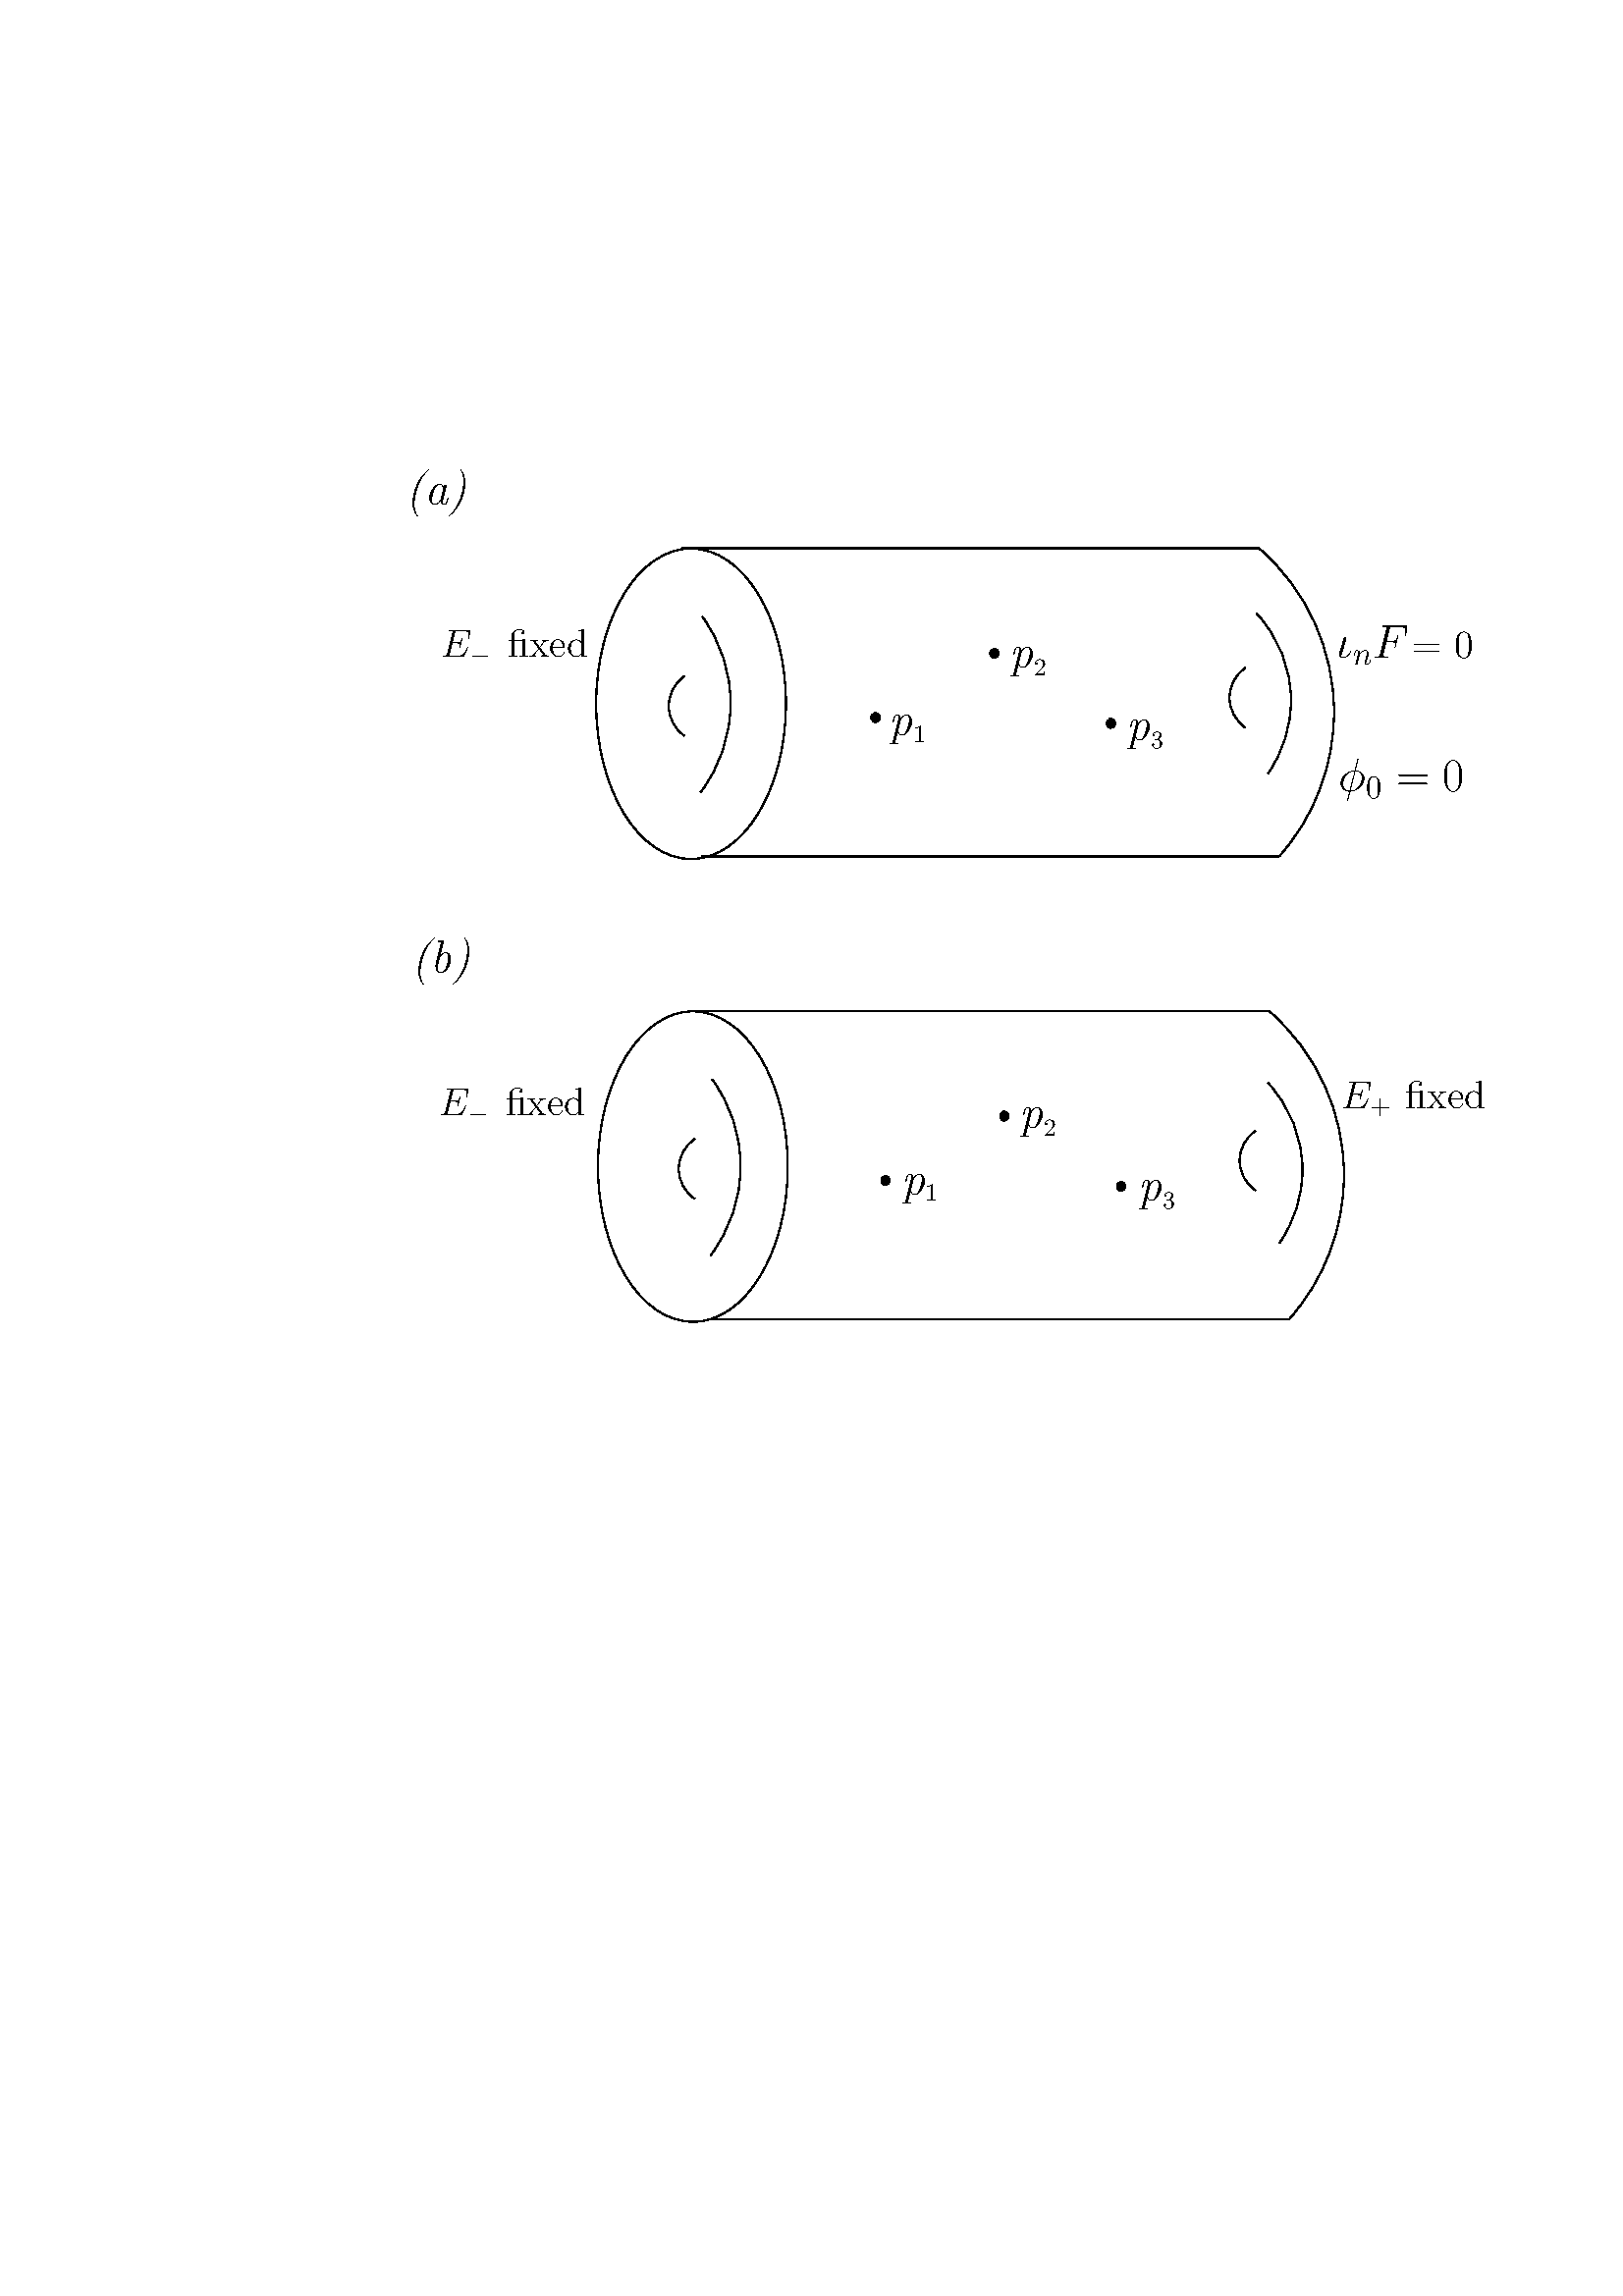
\includegraphics[width=0.75\linewidth]{figures/gla7-4.png}
\caption{(a) 在带有 't Hooft 算子插入的三维流形 $W=I\times C$ 上，左端指定了一个丛 $E_-$，人们希望确定右端可能出现的 Hecke 修正 $E_+$。左端联络 $A_-$ 满足 Dirichlet 边界条件，$\phi_0$ 未加指定；右端则相反。(b) 为描述 Hecke 对应的纤维，需要同时指定 $E_-$ 与 $E_+$，并在两端都让 $\phi_0$ 未加指定。（原文 Fig.~15）}
\label{fig:utampo}
\end{figure}

我们可能考虑两个密切相关的问题。一个自然的问题是描述 't Hooft/Hecke 算子对丛的作用，第二个是描述 Hecke 对应。

对第一个问题（\utampo(a)），我们在 $W$ 的左端指定一个丛 $E_-$，然后问：通过解带奇点的 Bogomolny 方程，另一端能出现什么样的丛 $E_+$。这样我们应当能重新得到 Hecke 修正空间，如第~\ref{sec:theck}~节 所描述。另一个可选的问题（\utampo(b)）是试图描述 Hecke 对应，它参数化具有适当 Hecke 关系的丛配对。我们将描述适合这两个问题中任何一个的边界条件。

为指定丛 $E_-$，我们指定 $C_-$ 上的规范场 $A_-$。我们要指定的是实际的丛 $E_-$，而不是丛的同构类，所以我们指定 $C_-$ 上一个实际的联络 $A_-$。因此我们只模去那些在 $C_-$ 上为平凡的规范变换。对某些目的而言，方便的做法是假定丛 $E_-$ 稳定，此时可以假定联络 $A_-$ 平坦。我们不假定由解 Bogomolny 方程得到的输出丛 $E_+$ 稳定。

\begin{yizhu}[易错点]
按：这里指定的是 $C_-$ 上一个具体的联络 $A_-$，而不是丛的同构类，因此只模去在 $C_-$ 上为平凡的规范变换；若两端都模去规范变换，得到的对象是 ${\rm Bun}_G$ 上的点而不是给定 $E_-$ 的 Hecke 修正空间。$E_-$ 稳定的假定只是为了能取平坦代表，输出丛 $E_+$ 并未假定稳定。
\end{yizhu}

我们希望 $C_-$ 上的边界条件（在模去规范变换后）是椭圆的。Bogomolny 方程中最简单的椭圆边界条件是：要么对 $A$ 施加 Dirichlet 边界条件（即指定其边界值）而不指定 $\phi_0$ 的边界值，要么反过来。若指定了 $A$ 的边界值，则 Bogomolny 方程会确定 $\phi_0$ 在边界处的法向导数；反之亦然。在 $E_-$ 处，由于我们要指定 $A$，就令 $\phi_0$ 不加指定。若 $A_-$ 平坦，则 Bogomolny 方程要求在 $C_-$ 处 $\phi_0$ 的法向导数为零。

另一方面，在 $C_+$ 处，我们希望允许由 $E_-$ 经解 Bogomolny 方程可能出现的一切 Hecke 修正 $E_+$。所以 $C_+$ 上不指定联络 $A$，而是令 $C_+$ 上 $\phi_0=0$。于是 Bogomolny 方程要求 $A$ 在 $E_+$ 处满足协变 Neumann 边界条件；即其曲率 $F(A)$ 与边界的法向量缩并时为零。我们只关心模去规范变换的输出丛 $E_+$，所以允许规范变换在 $C_+$ 上非平凡。这些边界条件总结在 \utampo(a) 中。在第~\ref{sec:kahstr}~节 中，我们将更深入地理解这些边界条件的自然性。

\begin{yizhu}[物理图像]
按：$C_+$ 端令 $\phi_0=0$ 而让 $A$ 自由（协变 Neumann），与 $C_-$ 端的 Dirichlet 条件恰好互补：Bogomolny 方程是椭圆系统，每端只需在「指定 $A$」与「指定 $\phi_0$」之间二选一，就能得到椭圆问题。$C_+$ 端不指定 $A$，正是为了让所有可能的 Hecke 修正都能出现；若把 $A_+$ 也固定，得到的便是 Hecke 对应在配对 $(A_-,A_+)$ 上的纤维（见下文 \utampo(b)）。
\end{yizhu}

\par\medskip{\it Hecke 对应}

我们刚才描述的是在用 Bogomolny 方程研究 Hecke 算子时一般会采用的边界条件。但我们要停下来讨论一下代数几何中另一种标准表述的微分几何类比。（本文余下部分并不需要这些细节。）与上面把 $E_-$ 看作输入、$E_+$ 看作输出不同，人们可以对称地处理两者，办法是描述「Hecke 对应」。在代数几何的通常表述中，令 ${\rm Bun}_G$ 为 $C$ 上所有 $G$-丛构成的「栈」，不要求稳定。型为 $^L\negthinspace w,z$ 的 Hecke 对应（$^L\negthinspace w$ 是权，$z\in C$ 是点）则是一个簇 ${\cal Q}(^L\negthinspace w,z)$，它映到 ${\rm Bun}_G\times {\rm Bun}_G$。${\cal Q}(^L\negthinspace w,z)$ 在 $E_-\times E_+\in {\rm Bun}_G\times {\rm Bun}_G$ 上的纤维，参数化了在 $z$ 处用型 $^L\negthinspace w$ 的 Hecke 变换把 $E_-$ 变到 $E_+$ 的各种方式。


$E_-$ 与 $E_+$ 之间的关系可以更对称地表述，因为 $C_-$ 与 $C_+$ 由一个保向自同构 ${\cal PT}$ 互换：它在 $C$ 上作用平凡，交换 $I$ 的两端，并且反转时间坐标。这样的自同构把 $\phi$ 映到 ${\cal PT}^*(\phi)$，并把权为 $^L\negthinspace w$ 的 't Hooft 算子映到权为 $^L\negthinspace w'$ 的算子，其中 $^L\negthinspace w'$ 是与 $-{}^L\negthinspace w$ Weyl 共轭的支配权。因此，$E_+$ 由 $E_-$ 经 $z$ 处型 $^L\negthinspace w$ 的 Hecke 变换得到，等价地，$E_-$ 由 $E_+$ 经 $z$ 处型 $^L\negthinspace w'$ 的 Hecke 变换得到。

若权 $^L\negthinspace w$ 较小而 $C$ 的亏格较大，则映到 ${\rm Bun}_G\times {\rm Bun}_G$ 的映射 ${\cal Q}({}^L\negthinspace w,z)$ 的纤维一般是空的。另一方面，若 $^L\negthinspace w$ 足够大，则对任何 $C$ 这个映射一般是纤维化。可以把 ${\cal Q}$ 的定义推广到允许若干具有指定位置与权的 Hecke 算子，此时映射 ${\cal Q}\to {\rm Bun}_G\times {\rm Bun}_G$ 的性质取决于 't Hooft 算子的数目与权。

在微分几何中，${\rm Bun}_G$ 对应于所有联络构成的空间 $\EUA$。$\EUA$ 当然是无穷维的，而 ${\rm Bun}_G$ 是无穷维流形的代数几何类比（它包含任意不稳定的丛，形变空间与自同构群的维数都没有界）。Hecke 对应 ${\cal Q}$ 同样是无穷维的，不会来自椭圆边界条件。Hecke 对应的微分几何版本就是直接把 ${\cal Q}$ 定义为 $W=I\times C$ 上带指定奇点的 Bogomolny 方程所有解构成的空间，模去在两端均为平凡的规范变换。把 ${\cal Q}$ 映到 $\EUA\times \EUA$ 的映射，由把解限制到 $W$ 的两端得到。

${\cal Q}$ 是无穷维的，因为我们在定义它时两端都没有指定 $A$ 或 $\phi_0$；这些边界条件不是椭圆的。在微分几何中，更自然的做法是定义 Hecke 对应在一对联络 $A_-\times A_+\subset \EUA\times \EUA$ 上的纤维。这就是在代数几何中研究映射 ${\cal Q}\to {\rm Bun}_G\times {\rm Bun}_G$ 的纤维的规范理论类比。为此，我们在两端分别固定 $A_-$ 与 $A_+$，并模去在两端均为平凡的规范变换（\utampo(b)）。带这些边界条件的 Bogomolny 方程所有解构成的空间，就是 Hecke 对应在配对 $A_-\times A_+$ 上的纤维。定义这个纤维的边界条件是椭圆的，它相当于在 $W$ 的两端都采用在 \utampo(a) 中只加在 $C_-$ 上的边界条件。

Hecke 对应纤维的虚拟复维数可以用指标理论、通过修改下面给出的讨论来计算。它等于 $-(g-1){\rm dim}(G)$ 加上型 $^L\negthinspace w$ 的 Hecke 修正空间的维数 $\Delta$（也在下面计算）。若虚拟维数是负数 $-d$，意味着 ${\cal Q}$ 一般是 $\EUA\times \EUA$ 中余维为 $d$ 的子簇。若它是正整数 $d'$，意味着 ${\cal Q}$ 一般以维数为 $d'$ 的纤维纤维化于 $\EUA\times \EUA$ 之上。

然而，在余下的分析中，我们集中描述给定丛 $E_-$ 的可能 Hecke 修正构成的空间，因此采用 \utampo(a) 的边界条件。在研究更详细的性质之前，我们先看看能从指标理论学到什么。

\par\medskip{\it 指标理论与虚拟维数}

令 ${\EUZ}$ 为带 \utampo(a) 的椭圆边界条件的 Bogomolny 方程解的模空间。由我们在第~\ref{sec:thooftheckeop}~节 对 't Hooft 算子与 Hecke 算子关系的讨论，可以预期 ${\EUZ}$ 是复流形。我们将在第~\ref{sec:kahstr}~节 证明这一点。Bogomolny 方程的线性化给出 \cite{ref107,ref108} 中研究过的椭圆复形：
% 式 (10.1)
\setcounter{equation}{0}
\begin{equation}\label{eq:tifor}
0\to \Omega^0({\rm
ad}(E))\underarrow{~d_1~}\Omega^1({\rm ad}(E))\oplus \Omega^0({\rm
ad}(E))\underarrow{~d_2~}\Omega^2({\rm ad}(E))\to 0 .
\end{equation}
（这里 $\Omega^i({\rm ad}(E))$ 是取值于 ${\rm ad}(E)$ 的 $i$-形式构成的空间。$d_1$ 是把 $\Omega^0({\rm ad}(E))$（规范变换的 Lie 代数）的元素映到 $A$ 与 $\phi$ 的线性化的映射，其像分别取值于 $\Omega^1({\rm ad}(E))$ 与 $\Omega^0({\rm ad}(E))$。$d_2$ 是 Bogomolny 方程的线性化。）${\EUZ}$ 的切空间是这个复形的一阶上同调群，即 $ H^1={\rm ker}(d_2)/{\rm im}(d_1)$。这个椭圆复形的指标称为 ${\EUZ}$ 的虚拟维数；若其他上同调群 $H^0={\rm ker}(d_1)$ 与 $H^2={\rm coker}(d_2)$ 为零，则它与实际维数一致。$H^0$ 由 $\Omega^0({\rm ad}(E))$ 的协变常值截面组成，它们生成未破缺的规范对称性。在我们的边界条件下，$H^0$ 为零，因为我们要求规范变换在 $W$ 的一端为平凡。如我们将看到的，在 \utampo(a) 的边界条件下，虚拟维数非负。既然如此，$H^2$ 在 ${\EUZ}$ 的奇点之外为零，而 ${\EUZ}$ 的光滑部分是一个流形，其维数等于虚拟维数，即该复形的指标。

\begin{yizhu}[易错点]
按：$H^2$ 的消灭是「虚拟维数＝实际维数」的前提，而 $H^0$ 的消灭则来自边界条件：我们要求规范变换在 $W$ 的一端为平凡，等价于不把两端的规范变换都当作冗余。若在两端都模去规范变换，$H^0$ 会非零，指标与模空间维数就不再一致。另外，$H^2$ 只在 ${\EUZ}$ 的奇点处可能不为零，所以光滑部分确实是维数等于指标的流形。
\end{yizhu}

我们首先分析没有任何 't Hooft 算子时的 Bogomolny 方程。为简单起见，假定 $E_-$ 稳定，并由一个 $F=0$ 的平坦联络代表。（总可以形变到这种情形而不改变指标。）在这种情况下，一种标准的论证表明：带上述任何边界条件的 Bogomolny 方程的解都是从 $C$ 拉回的解，因此特别地 $E_+$ 与 $E_-$ 同构。这其实是第~\ref{sec:vanishing}~节 消灭定理的一个特例，但论证非常简单，我们在此单独给出。

若满足 Bogomolny 方程 $F-\star D\phi_0=0$，则 $0=\int_W\Tr\,(F-\star D\phi_0)\wedge \star (F-\star D\phi_0)$。把它展开并分部积分，得到
% 式 (10.2)
\setcounter{equation}{1}
\begin{equation}\label{eq:notty}
-\int_W\Tr\,\left(F\wedge\star F+D\phi_0 \wedge \star
D\phi_0\right)=-2\int_{\partial W}\Tr\,\phi_0 F.
\end{equation}
边界项在 $\partial W$ 上使 $\phi_0$ 或 $F$ 为零的那个分支上消失。在 \utampo(a) 中，一端有 $F=0$，另一端有 $\phi_0=0$，所以边界项在两端都消失。但 \eqref{eq:notty}\ 的左端是半正定的，只有当 $F=D\phi_0=0$ 时才能为零。因此，在 $E_-$ 平坦的假定下，带这些边界条件且没有 't Hooft 算子的任何 Bogomolny 方程解，都是由从 $C$ 拉回的、$\phi_0=0$ 的平坦联络给出。

特别地，$E_+$ 同构于 $E_-$，而 ${\EUZ}$ 是一个点，维数为零。还可以进一步验证，在带 \utampo(a) 边界条件的这种平凡解附近展开时，$H^2$ 为零。所以在这种情况下，${\EUZ}$ 的虚拟维数与实际维数相同，即零。那么，若把 't Hooft 算子包括进来会怎样？与 't Hooft 算子 $T(^L\negthinspace R)$ 相关联的每个奇点，都把模空间的虚拟维数平移一个量，而这个量只依赖于对偶群的表示 $^L\negthinspace R$（不依赖于 't Hooft 算子所插入的三维流形的细节、丛 $E$ 的拓扑，或其他 't Hooft 算子的可能存在）。这由指标理论的一般切除性质 \cite{ref123} 可得，Pauly \cite{ref124} 证明了它。此外，用我们的语言，Pauly 计算了 't Hooft 算子对模空间维数的贡献，情形为 $G=PSU(2)=SO(3)$、$^L\negthinspace G=SU(2)$。答案\footnote{这是 \cite{ref124} 的定理 I，其中 $k$ 对应于我们所称的 $a/2$。该定理对偶数 $a$ 陈述，因为规范群取为 $G=SU(2)$ 而非 $PSU(2)$，但其证明对奇数 $a$ 也成立，事实上对所有 $G$ 都成立，如我们将讨论的。}是：与最高权 $^L\negthinspace w=(a/2,-a/2)$（$a$ 为正整数）的表示相关联的 't Hooft 算子，把 Bogomolny 方程解的模空间 ${\EUZ}$ 的虚拟（复）维数平移 $a$。

奇点把复维数增加 $a$ 这一事实，与我们第~\ref{sec:spaceheck}~节 通过考察 Hecke 修正空间得到的结果一致。在那里我们证明了：对 $U(2)$ 的权 $(a,0)$，等价地对 $SU(2)$ 的权 $(a/2,-a/2)$，Hecke 修正空间的复维数为 $a$。

Pauly 的证明其实可以直接推广到任意紧 Lie 群 $G$。为解释这一点，我们必须回顾 Pauly 证明背后的技巧，它由 Kronheimer \cite{ref110} 引入。基本想法是考虑四维流形\footnote{Kronheimer 实际上考虑了更一般的情形：把 $\Bbb{C}^2$ 换成更一般的带 $U(1)$ 作用的四维超凯勒流形，并得到 $\Bbb{R}^3$ 上具有更一般奇点集的 Bogomolny 方程解的描述。} $\Bbb{C}^2\cong \Bbb{R}^4$ 上在 ${\EUF}=U(1)$ 作用 $(z_1,z_2)\to (\exp(i\theta)z_1,\exp(i\theta)z_2)$ 下不变的瞬子。商 $\Bbb{C}^2/{\EUF}$ 同构于 $\Bbb{R}^3$。${\EUF}$ 的作用并不自由——它在原点 $z_1=z_2=0$ 处有不动点——但尽管如此，商 $\Bbb{C}^2/{\EUF}$ 仍是流形 $\Bbb{R}^3$。从 $(z_1,z_2)\in \Bbb{C}^2$ 到 $\vec x\in \Bbb{R}^3$ 的映射为

\begin{yizhu}[原文疑误]
按：原文此处脚注写「solutions of the Bogomolny solutions on $\Bbb{R}^3$」，其中第二个 solutions 应为 equations，即「$\Bbb{R}^3$ 上 Bogomolny 方程的解」。译文按后一意思译出；这是作者笔误，语法上也无从解释。
\end{yizhu}

\begin{yizhu}[物理图像]
按：Kronheimer 的技巧把四维的 $U(1)$-不变瞬子与三维的 Bogomolny 方程解对应起来：$U(1)$ 在 $\Bbb{C}^2$ 上的作用有不动点，商 $\Bbb{C}^2/U(1)\cong\Bbb{R}^3$，而不动点纤维上的同态 $\rho:U(1)\to G$ 决定 't Hooft 算子的型。Pauly 据此把「奇点对指标的贡献」化为「不动点对等变指标的贡献」，这是等变指标定理的固定点公式（局部化）的标准应用。
\end{yizhu}
% 式 (10.3)
\setcounter{equation}{2}
\begin{equation}\label{eq:nigo}
\vec x=\bar z\vec\sigma z,
\end{equation}
其中 $\vec\sigma$ 是 $2\times 2$ 无迹 Hermite 矩阵（归一化为 $\Tr\,\sigma_i\sigma_j=2\delta_{ij}$，即著名的 Pauli 自旋矩阵）。这提示 $\Bbb{C}^2$ 上 ${\EUF}$-不变的瞬子可能与 $\Bbb{R}^3$ 上有趣的对象有关，但应当预期在 $\Bbb{R}^3$ 的原点（对应于 $\Bbb{C}^2$ 原点处的不动点）会发生某种特别的事情。

$\Bbb{C}^2$ 上 ${\EUF}$-不变瞬子的描述有些微妙。若把 ${\EUF}$ 在 $\Bbb{C}^2$ 上的作用提升为对 $G$-丛 $\hat E\to \Bbb{C}^2$ 的作用，则特别地 ${\EUF}$ 作用在 $\hat E$ 于不动点处的纤维 $\hat E_{0}$ 上。这样的作用由同态 $\rho:{\EUF}\cong U(1)\to G$ 刻画。我们回忆，这样的同态可以解释为 $^L\negthinspace G$ 的一个权，并确定一个 't Hooft 算子 $T(\rho)$。Kronheimer 考虑 $\Bbb{C}^2$ 上给定 $\rho$ 的 ${\EUF}$-不变瞬子，并证明它们等价于 $\Bbb{R}^3$ 上在原点有奇点的 Bogomolny 方程解，而这个奇点用我们的语言表示算子 $T(\rho)$ 的插入。

Pauly 进而证明：型为 $\rho$ 的奇点对 ${\EUZ}$ 虚拟维数的贡献 $\Delta_\rho$，可以由 $\Bbb{C}^2$ 原点处不动点对「计算 $\Bbb{C}^2$ 上瞬子形变的线性算子」的 ${\EUF}$-等变指标的贡献算出。令 ${\rm ad}(\hat E)$ 为由 $\hat E$ 导出的伴随丛，${\rm ad}(\hat E)_0$ 记它在原点的纤维。不动点对指标的贡献涉及 ${\rm ad}(\hat E)_0$ 中的一个迹。（伴随表示出现，是因为瞬子的形变理论涉及一个作用在伴随丛上的椭圆算子。）按照 Pauly 在第 4.2 节中的计算，结果可以描述如下。${\EUF}\cong U(1)$ 在 ${\rm ad}(\hat E)_0$ 上的作用（由 $\rho:{\EUF}\to G$ 与 $G$ 的伴随表示复合得到）分解为特征之和。${\EUF}$ 的任何特征都形如 $\exp(i\theta)\to \exp(im\theta)$，其中 $m$ 是某个整数。由于 $G$ 的伴随表示是实表示，$\rho$ 分解成特征时出现的非零整数成对出现 $c_k,-c_k$，其中可取 $c_k$ 为正。于是 't Hooft 算子 $T(\rho)$ 对 ${\EUZ}$ 虚拟维数的贡献为
% 式 (10.4)
\setcounter{equation}{3}
\begin{equation}\label{eq:xinon}
\Delta_\rho=\sum_kc_k.
\end{equation}
这推广了 $G=PSU(2)$ 的情形，那里只出现一个整数 $c$。Pauly 的分析立刻从 $SU(2)$ 推广到任意 $G$，因为等变指标定理对任意 $G$ 都成立。计算涉及 Lie 代数中的一个迹，由此得到 \eqref{eq:xinon}。

完全不带 't Hooft 算子时，我们的边界条件下的虚拟维数为零。所以带单个 't Hooft 算子 $T(\rho)$ 时，虚拟维数为 $\Delta_\rho$。但带单个 't Hooft 算子时，${\EUZ}$ 恰好就是型为 $\rho$ 的 Hecke 修正空间 ${{\EUY}}(\rho)$。Hecke 修正空间维数的公式 \eqref{eq:xinon}\ 与 $U(N)$（或 $SU(N)$ 或 $PSU(N)$）的结果 \eqref{eq:ydro}\ 一致，并将它推广到任意的紧群 $G$。

由于 't Hooft 算子对指标理论的贡献是局部的，我们可以立刻写出下述一般结果：带任意指定的一组 't Hooft 算子插入时，Bogomolny 方程解的模空间 ${\EUZ}(\rho_1,\dots,\rho_n)$ 的维数。若没有 't Hooft 算子，${\EUZ}$ 的维数为零。每个与同态 $\rho_i:U(1)\to G$ 相关联的 't Hooft 算子 $T(\rho_i)$ 对维数贡献 $\Delta_{\rho_i}$，所以一般地 ${\EUZ}(\rho_1,\dots,\rho_n)$ 的维数为
% 式 (10.5)
\setcounter{equation}{4}
\begin{equation}\label{eq:migoty}
\Delta=\sum_i\Delta_{\rho_i}.
\end{equation}
